\chapter{Arithmetic Circuits}

A library of commonly used arithmetic functions is needed for implementing a
basic set of built in functions in a reversible compiler.  Extra consideration
is given to in-place functions whenever possible due to the improved efficiency
provided by reversible mutation in MDD based cleanup.

This section also demonstrates the usefulness of pebble based circuit analysis.
It is possible, using pebble games, to achieve an asymptotic improvement over
previous results in the space-time product for reversible Karatsuba.

\section{Addition}

  An addition circuit is a circuit which takes two $n$ bit integers $\mathbf{a} =
  a_1a_2\dotsc a_n$ and $\mathbf{b} = b_1b_2\dotsc b_n$ and returns the sum
  $\mathbf{a}+\mathbf{b}\mod 2^n$. The operation $(a,b)\mapsto (a,a+b)$ is injective so
  it is expected that an addition circuit which is in-place on one of its input exists.

  \subsection{Classic Ripple}

    The classic ripple addition method simply adds the bits in each column
    starting from the least significant bit.  The output for that bit is the
    result modulo 2 and a carry is set to be added to the next column if the
    result is $>1$.

    To perform this algorithm we will need a circuit which takes three bits then
    calculates the carry and sum.  These can then be applied iteratively taking
    the two bits from each column of the numbers that are to be added as well as
    the previous carry.

    This can be done with a full adder circuit.  A full adder is a circuit
    which takes input bits $a$, $b$, and $c$ then returns the sum ($a \oplus b
    \oplus c$) as well as the carry ($ab\oplus ac \oplus bc$).
    \Cref{fig:classicalFA} shows an irreversible implementation.

    \begin{figure}
        \capstart
        \centering
        
\includegraphics[width=0.5\textwidth]{images/classicalFA.pdf}
        \caption{Irreversible full adder.}
        \label{fig:classicalFA}
    \end{figure}
    In the reversible case a circuit (see figure~\ref{fig:reversibleFA}) can be constructed that performs the mapping:
    \[
        (a,b,c,0) \mapsto (a,b,a\oplus b\oplus c,ab\oplus ac \oplus bc)
    \]
    \begin{figure}[ht]
        \capstart
        \centering
        \[
          \Qcircuit @C=1em @R=.7em {
              \lstick{a} & \ctrl{3} & \qw      & \ctrl{1} & \qw      & \rstick{a}\qw\\
              \lstick{b} & \targ    & \ctrl{2} & \targ    & \ctrl{1} & \rstick{b}\qw\\
              \lstick{c} & \targ    & \ctrl{1} & \qw      & \targ    &\rstick{a  \oplus b  \oplus c}\qw\\
              \lstick{0} & \targ    & \targ    & \qw      & \qw      &\rstick{ab \oplus ac \oplus bc}\qw
          }
        \]
        \caption{Reversible full adder\cite{tomAdder}. Partially in place since $c$ is overwritten.}
        \label{fig:reversibleFA}
    \end{figure}

    These can then be chained together as they are in the irreversible case.
    The result will be a circuit which takes inputs $(a,b)$ and produces
    outputs $(a,b,a+b)$.  Note that since a Toffoli gate can be implemented in
    T-depth one\cite{selinger2013} an out-off-place adder can be implemented in
    T-depth $n$ where $n$ is the bit width of its inputs.

\subsection{In-Place Ripple}

    It is sometimes the case that one of the input values is unneeded after the
    operation.  In that case it would save space to overwrite the value.  To do
    this we could try to construct an adder which implements the injective map
    $(a,b)\mapsto(a,a+b)$.

    Such an adder is described Cuccaro et. al. in \cite{CDKM:2004} (Note that
    not all the optimizations described in the original paper are desirable
    with our gate set as we wish to maximize shared controls).  It is very
    similar to the classic ripple, the main improvement is the realization
    that information about the carry could be stored in one of the input bits
    of each column.  This allows it to overwrite one of its inputs with the
    resulting sum.  The circuit uses two main operations: MAJ, and UMA (See
    \cref{fig:majuma}).  The MAJ operation takes an input carry $c$ and two
    input bits $a$ and $b$.  It computes the carry onto $a$ and partially
    computes the sum on $b$, it leaves $c$ in an unclean state to be fixed
    later.  This circuit can be repeated and rippled through all of the
    columns.  After that is done the UMA operation can be performed.  This
    operation cleans up $a$ and $c$ then finishes computing the sum on $b$.

    \begin{figure}[ht]
        \capstart
        \centering
        \begin{subfigure}{.45\textwidth}
            \centering
            \[
              \Qcircuit @C=1em @R=.7em {
                 \lstick{c} & \qw          & \targ      & \ctrl{2} & \rstick{c \oplus a}\qw\\
                 \lstick{b} & \targ        & \qw        & \ctrl{1} & \rstick{b \oplus a}\qw\\
                 \lstick{a} & \ctrl{-1}    & \ctrl{-2}  & \targ    & \rstick{ab \oplus ac \oplus bc}\qw
              }
            \]
            \caption{MAJ}
        \end{subfigure}
        \begin{subfigure}{.45\textwidth}
            \centering
            \[
              \Qcircuit @C=1em @R=.7em {
                  & \ctrl{2} & \targ      & \ctrl{1} & \rstick{c}\qw\\
                  & \ctrl{1} & \qw        & \targ    & \rstick{a \oplus b \oplus c}\qw\\
                  & \targ    & \ctrl{-2}  & \qw      & \rstick{a}\qw
              }
            \]
            \caption{UMA}
        \end{subfigure}
        \caption{Basic operations used in the adder.}
        \label{fig:majuma}
    \end{figure}

    The cost of this adder is $2n-2$ Toffoli gates for an adder $\mod 2^n$.
    Note that each Toffoli gate has two shared controls which means it is
    possible to cancel at least two T-gates per Toffoli.

    %\todo{Further reductions may be possible using T-par}

\subsection{Controlled Ripple}

    This is a simple Controlled addition circuit with a gate count and depth
    $\Theta(n)$.  Note that not all gates need be controlled; controlling a set
    of gates which if removed would transform the circuit into the identity is
    sufficient\footnotemark. In the case of the in-place adder the MAJ and UMA subcircuits
    can be made to cancel by removing one gate each. \Cref{fig:ctrlRipple}
    shows the resulting circuit.

    \footnotetext{Let $U_{\text{ctrl}}$ denote a controlled $U$ operation. The
    simplest example of this is $W=UVU^{-1}$. Here we can construct
    $W_{\text{ctrl}} = UV_{\text{ctrl}}U^{-1}$. As a slightly more complex example
    say $ABC=I$ and $X=AYBZC$ then $X_{\text{ctrl}} = AY_{\text{ctrl}}BZ_{\text{ctrl}}$.}

    \begin{figure}[ht]
      \capstart
      \centering
      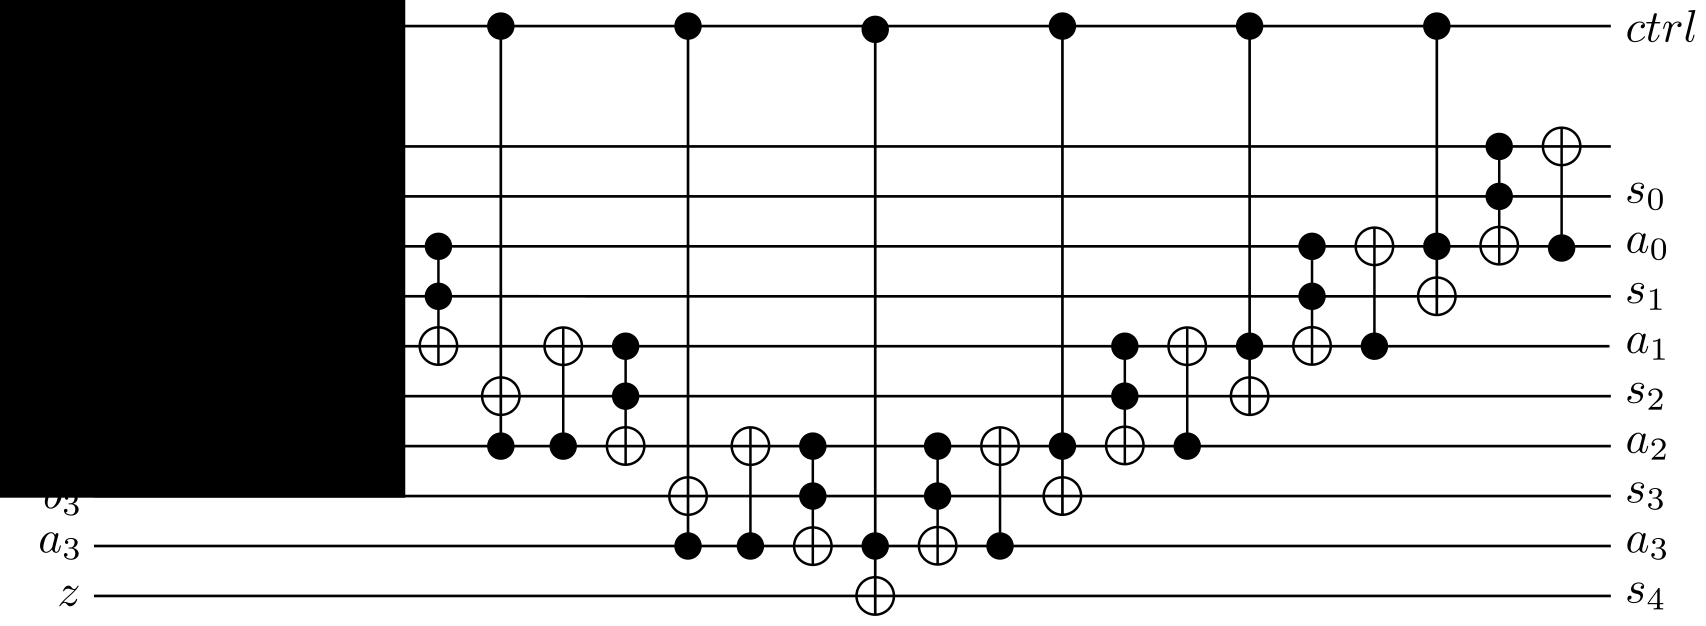
\includegraphics[width=\textwidth]{images/4BitRippleAdderCtrl}
      \caption{Controlled In-Place Ripple Adder. Based on the adder from \cite{CDKM:2004}. }
      \label{fig:ctrlRipple}
    \end{figure}
    \subsection{Analysis}

      This modification can be accomplished by changing $2n+1$ CNOT gates into
      Toffoli gates.  This gives a controlled addition circuit of size $n$
      ($A^{ctrl}_n$) a total gate count:

      \begin{align} \label{eq:cadd}
        A^{ctrl}_n = 4n+1
      \end{align}

\section{Multiplication}
  \subsection{Controlled Addition Multiplier}

    A very simple implementation of multiplication, which is described in
   \cite{offermann2010} uses controlled addition circuits (see
   \cref{fig:ctrlRipple}). Given two numbers as bit strings $a$ and $b$ their
   product can be found by repeatedly shifting forward by one and adding $b$ to
   the result controlled on the next bit in $a$.  See \cref{fig:multAdd} for a
  four bit example. This is essentially the elementary school shift and add
  method of multiplication on binary numbers. It is out of place and uses only
  one additional ancilla for the adder circuits.

    \begin{figure}[ht]
      \capstart
      \centering
      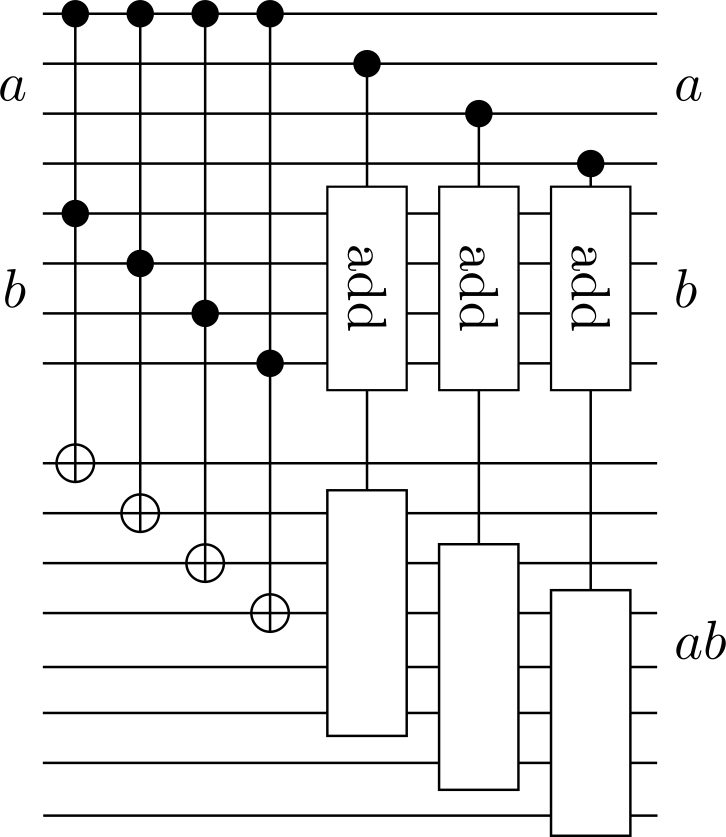
\includegraphics[scale=0.25]{images/multCtrlAdd}
      \caption{Controlled Addition Multiplier. Triangles are used in this figure to show which bits are modified by the adder.}
      \label{fig:multAdd}
    \end{figure}
    \subsubsection{Analysis}
      This circuit takes $n$ Toffoli gates to copy down the initial value.
      It then uses $n-1$ controlled in place addition circuits to produce the final value.

      So if we define $A^{ctrl}_n$ to be the Toffoli count for a controlled adder of size $n$ we get $M_n = n + (n-1)A^{ctrl}_n$
      Where $M_n$ is the gate count for a controlled addition based multiplication circuit of size $n$.
      From \eqref{eq:cadd} we know the controlled addition circuit uses $4n+1$ Toffoli gates this gives a full count:
      \begin{align} \label{eq:caddtoff}
        M_n = 4n^2 - 2n -1
      \end{align}

  \subsection{Reversible Karatsuba\label{sec:kara}}    
    Let $n\geq 1$ and let $x$ and $y$ be $n$-bit integers.  The
    Karatsuba\cite{KO:1963} algorithm is based on the observation that by
    writing $x=x_1 2^{\lceil n/2\rceil}+x_0$ and $y=y_1 2^{\lceil n/2\rceil
    }+y_0$ the product $xy$ can be evaluated as $xy=2^n A + 2^{\rceil n/2
    \rceil} B + C$, where

The following reversible algorithm for Karatsuba improves upon previous
work\cite{PF:2006,Kepley2015,offermann2010}. An asymptotic improvement is space
use (yielding as well an asymptotic improvement in the space-time product), is
shown by using pebble games in the analysis. Further some constant improvements
are realized by using in place addition to minimize garbage growth at each
level and by optimally splitting the input in each recursive step rather then
just dividing the bit-string in half, this is helpful when the integer size is
not a power of 2.

    \begin{align*}
      A &= x_1 y_1, \\
      B &= (x_0+x_1)(y_0+y_1) - x_0 y_0 - x_1 y_1,\\
      C &= x_0 y_0. \\
    \end{align*}
    \begin{figure}[ht]
      \capstart
      \centering
      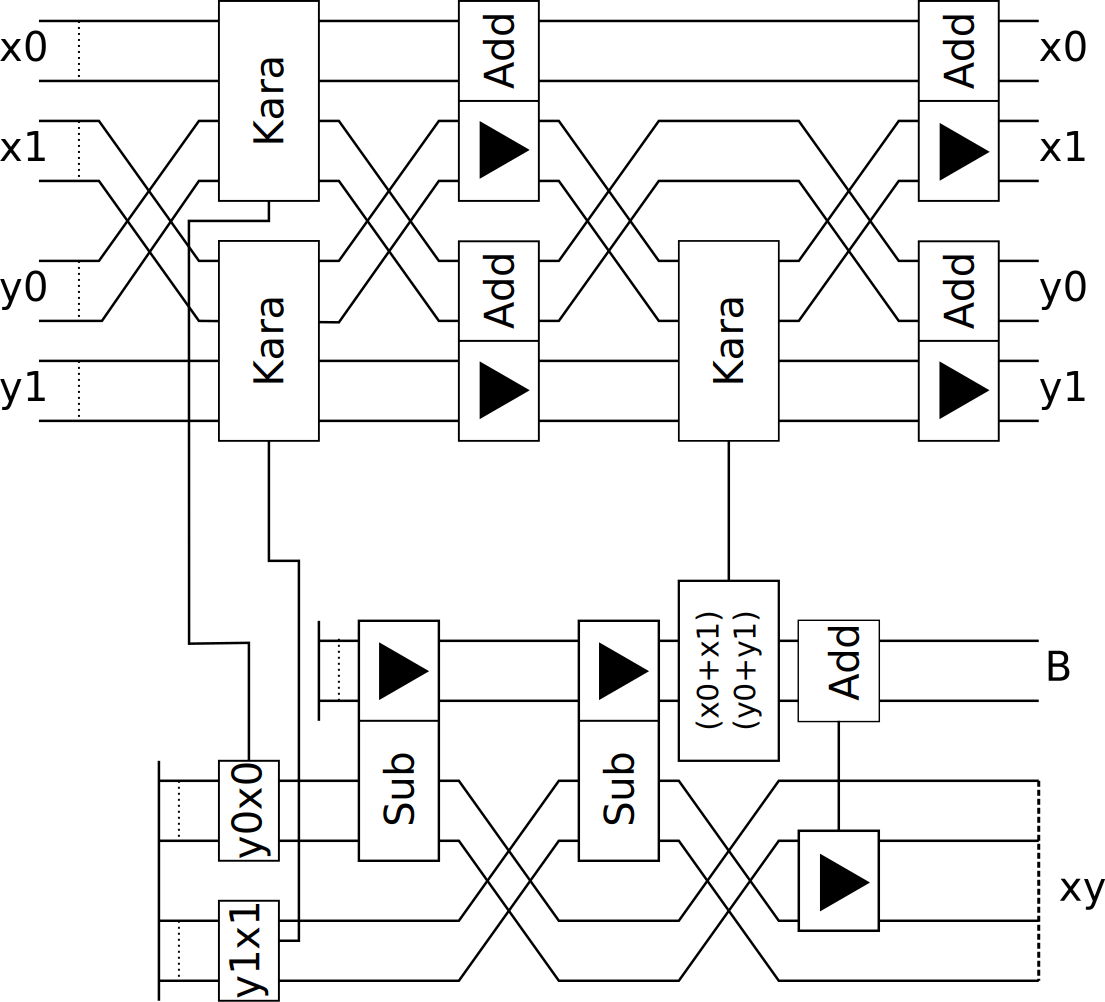
\includegraphics[width=2\textwidth/3]{images/karatsuba2}
      \caption{Karatsuba Multiplication Circuit. Triangles are used in this figure to show which bits are modified by the adder.}
      \label{fig:kara2}
     \end{figure}

    \subsubsection{Analysis}%\todo{Maybe add an MDD for the circuit}

      Note that the cost for the computation of $A$, $B$, and $C$ are $3$
      multiplications and four additions.  Note further that the additions to
      compose the final result do not have to be carried out as the bit
      representation of $xy$ is the concatenation of the bit representations of
      $A$, $B$, and $C$.  For $m\geq 1$, let $M^{g}_m$ denote the Toffoli cost
      of a circuit that multiplies $m$-bit inputs $x$ and $y$ using ancillas,
      i.e., a circuit that maps $(x, y, 0, 0) \mapsto (x, y, g(x,y), xy)$,
      where $xy$ is a $2m$-bit output, and $g(x,y)$ is an garbage output on
      $k\geq 1$ bits.  Furthermore, denote by $A_m$ the cost for an (in-place)
      adder of two $m$-bit numbers.  It is known that $A_m$ can be bounded by
      at most $2m$ Toffoli gates. Let $K_n$ denote the number of Toffoli gates
      that arise in the quantum Karatsuba algorithm (See fig \cref{fig:kara2}).
      The outputs of one step of the recursion are $x_0$,$x_1$, $y_0$, $y_1$,
      $x_0y_0$, $x_1 y_1$, and $xy$.  It is easy to see that allowing garbage,
      $K_n^g$ can be implemented using $3$ multipliers of half the bit size,
      $4$ in-place adders of size $n$ and $4$ in place adders of size $n/2$
      (note the subtracters are just reversed adders).  The base case is a
      multiplier for two one-bit numbers which can be done with one Toffoli
      gate, i.e., $K_1^{g}=1$.  We obtain the following recursion:
      %\todo{Check these computations.}

      \begin{align}
        K_n^{g} = 3 K_{n/2}^{g} + 4 \left(A_{n} + A_{n/2}\right); \quad K_1^{g}=1.
      \end{align}

      For the overall clean implementation of the Karatsuba algorithm we first
      run this circuit forward, copy out the final result using $n$ CNOTs, and
      then run the whole circuit backward.  This leads to an overall cost of
      $K_n = 2 K_n^{g}$ and $n$ CNOTs.  For the moment we focus on the Toffoli
      cost only.  By expansion we obtain that:

      \begin{align}
        K_n^{g} &= 3^{\log_2(n)} K_1^{g} + 4\left( A_{n}+ A_{n/2} \right) + 12\left( A_{n/2}+ A_{n/4} \right)\notag\\
                & + \ldots + 4 \cdot 3^{\log_2(n)-1} \left(A_2 + A_1\right)
      \end{align}

      Using that the Toffoli cost of $A_{n/2^i}$ is $2n/2^i$, we obtain for
      the overall Toffoli cost the following bound:

      \begin{align}
        K_n &= 2\left(3^{\log_2 n } + 4 \sum_{i=0}^{\log_2 n - 1} 3^i 2(3n/2^i)\right)\notag\\
            &= 2n^{\log_2 3} + 48n \left(\frac{1- (3/2)^{\log_2 n}}{1-3/2}\right) \notag\\
            &= 2n^{\log_2 3} + 96n \left((3/2)^{\log_2{n}} -1\right) \leq 98 n^{\log_2{3}}
      \end{align}

      This bound can be improved by replacing the recursive call to Karatsuba
      with naive multiplication once a certain cut-off has been reached (i.e. once
      $n$ goes below some cutoff value).  Looking at \cref{fig:cutoff} we see a
      comparison of various cutoff values (the naive method is also plotted for
      reference).

      Another way to improve this algorithm is to attempt to choose more
      intelligent splits rather then always splitting the inputs in half at
      each level.  This is important because the bit length of the numbers we
      are adding together may not be a power of two so dividing the input
      bit-string in half at each level might not be optimal.  In
      \cref{fig:cutoff} the line plotted as \verb+AKara10+ shows the result of
      using the optimal splits at each level.  These were found by a simple
      dynamic program which evaluated the total gate size for every possible
      split at every level and chose the optimal ones.

      As using these methods we find an optimal cutoff value of 11 (see
      \cref{fig:cutoffs}).

      \begin{figure}[p]
        \capstart
        \includegraphics[width=\textwidth,height=0.4\textheight]{images/avgCutoffs.tikz}
        \caption{Average circuit size over the interval 50-500 for various cutoff values.}
        \label{fig:cutoffs}
      \end{figure}
      \begin{figure}[p]
        \capstart
        \includegraphics[width=\textwidth,height=0.4\textheight]{images/akara.tikz}
        \caption{Comparison of various cutoffs for the adaptive cutoff version.}
        \label{fig:aKara}
     \end{figure}

\subsubsection{Time-Space Trade-offs}

We see in \cref{fig:cutoff,fig:size} that there are trade-offs available
between circuits size and gate count available by changing the cutoff
value. A higher cut-off value value results in a larger naive
multiplication circuits which are much more space efficient.

The reversible pebble game may be used to gain an asymptotic improvement
in the space required to implement this algorithm. Note the tree structure of
the recursive dependencies shown in \cref{fig:kara-mdd}.  We find a level such
that the size of each nodes subtree is approximately equal to the size of all
nodes at that level and above. Then for each node at that level in sequence
compute the node and uncompute all nodes below it. Once all the nodes are
computed compute the rest of the tree.  This will result in an asymptotic
improvement in the amount of space used while only applying a constant
multiplier ($<2$) to the overall time.


For Karatsuba circuit on input of size $n$ at a level $x$ in the tree there are
$3^x$ nodes of size $2^{-x}n$ for a total cost of

\[
n\left(\frac{3}{2}\right)^x.
\]

So the total cost of the full tree is given by
\[
    n\sum_{i=0}^{N} \left(\frac{3}{2}\right)^i,
\]
where $N=\log_2 n$.

We would like to break this tree into approximately equal sized subtrees at
some level.  Each tree at that level will be computed then uncomputed leaving
only the top node. To minimize space we will choose the size of these subtrees
to be approximately equal to the remaining size of the tree above them. To
find the height $k$ of such a tree we set:

\[
    \sum_{i=0}^{N-k-1} \left(\frac{3}{2}\right)^i = \frac{1}{2^{N-k}}\sum_{i=0}^{k-1} \left(\frac{3}{2}\right)^i.
\]

Since this is a geometric series we can use the identity $\sum_{k=0}^{n-1} r^k
= \frac{1-r^n}{1-r}$ which holds for all $r$ and obtain

\begin{align*}
    \frac{1- \nicefrac{3}{2}^{N-k}}{1 - \nicefrac{3}{2}} &= \frac{1}{2^{N-k}}\frac{1- \nicefrac{3}{2}^{k}}{1 - \nicefrac{3}{2}}.
\end{align*}

Rearranging terms, we obtain

\begin{align*}
    1- \nicefrac{3}{2}^{N-k} &= 2^{k-N} - \frac{3^k}{2^N}.
\end{align*}

Since $k\leq N$ and since we want that $\nicefrac{3}{2}^{N-k} \geq
\frac{3^k}{2^N}$ a simple calculation shows that this will be the case for $k
\leq \frac{N}{ 2- \frac{\log 2}{\log 3}} = 0.731N$. The total space use without
this optimization is normally calculated as

\[
    n\sum_{k=0}^{\log_2 n - 1} \left(\frac{3}{2}\right)^k = n\frac{1-(\nicefrac{3}{2})^{\log_2 n}}{1-\nicefrac{3}{2}}.
\]

Which gives space use of $O(n(\nicefrac{3}{2})^{\log_2 n})$ which is
equivalent to $O(n^{\log_2 3})$ or approximately $O(n^{1.585})$
Using the above optimization we get space usage that can be bounded by
\[
    O(n(\nicefrac{3}{2})^{\frac{\log 3}{ 2\log 3 - \log 2}\log_2 n}) \approx O(n^{1.428}).
\]

To find the depth of the circuit note that each node at level $k$ must be
computed sequentially. At level $k$ the number of trees is
\[
    3^{\left(1-\frac{\log 3}{ 2\log 3 - \log 2}\right)\log_2 n}.
\]

Each tree is of depth :

\[
    \frac{n}{2^{1-\frac{\log 3}{ 2\log 3 - \log 2}}}
\]

This gives an overall depth for computing the $k$ level of:

\[
    n\left(\frac{3}{2}\right)^{\left(1-\frac{\log 3}{ 2\log 3 - \log 2}\right)\log_2 n} \approx n^{1.152}
\]

This gives a space-depth product in the fully parallel version of $n^{1+\log_2
3}$ which is the same

\subsection{Generalization to other recursions\label{sec:recpeb}}

Assume that we are given a function with input size $n$ which splits a problem
into $a$ subproblems of size $\nicefrac{n}{b}$ where total work done to
subdivide is $O(n)$. Then the overall work to compute the function for a
problem of size $n$ is given by:

\[
    n\sum_{i=0}^{N} \left(\frac{a}{b}\right)^i.
\]

Solving as above we have:
\[
    k \leq \frac{\log_b n}{ 2- \frac{\log b}{\log a}}.
\]

This means that our method is effective for recursive functions where the
number of sub-problems is greater than the problem size reduction factor. This
is intuitive since if the problem size reduction factor is equal to the number
of sub-problems then the sum over the space requirements of each node in a
given level will always be equal. So the strategy discussed above would only
give a constant factor space reduction.


By setting $b$ in $\log b / \log a$ equal to $1$ we get a square root reduction
in space. This should be compared with a pebble games for complete binary
graphs that was reported on in \cite{peb16} in which a similar recursive
structure was considered.



      \begin{figure}[p]
        \capstart
        \centering
        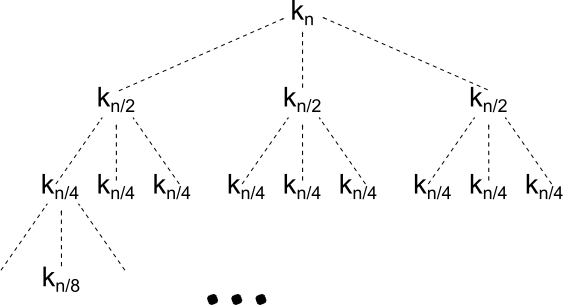
\includegraphics[width=0.7\textwidth]{images/kara-mdd}
        \caption{Structure of a pebble game for implementing the Karatsuba circuit. Note that $K_n$ can be implemented using $n/2+1$ ancilla.}
        \label{fig:kara-mdd}
      \end{figure}

     \begin{figure}[p]
        \capstart
        \includegraphics[width=\textwidth,height=0.4\textheight]{images/cutoff.tikz}
        \caption{Plot of circuit sizes vs input size for various various Karatsuba cutoffs.
                 The Legend shows the implementation (sKara for the simple version and aKara for the adaptive cutoff) as well as a number indicating the cutoff size. }
        \label{fig:cutoff}
      \end{figure}

      \begin{figure}[p]
        \capstart
        \includegraphics[width=\textwidth,height=0.4\textheight]{images/karaSize.tikz}
        \caption{Plot of bits used verses input size for various Karatsuba cutoffs.}
        \label{fig:size}
      \end{figure}
      \begin{figure}[p]
        \capstart
        \includegraphics[width=\textwidth,height=0.4\textheight]{images/karaDepth.tikz}
        \caption{Plot of Toffoli depth verses input size for various Karatsuba cutoffs.}
        \label{fig:depth}
      \end{figure}

\section{Division}
    In \cref{fig:div} is a simple integer division circuit based on the binary
    form of long division as outlined in \cref{algo:intdiv}.

    \noindent\begin{minipage}{.5\textwidth}
         \captionof{algorithm}{Integer Division with Remainder: find $R$ and $Q$ for $N/D$} \label{algo:intdiv}
         \begin{algorithmic}[1]
           \Require $D \neq 0$
           \State $Q \gets 0$
           \State $R \gets 0$
           \For{$i = n-1 \dots 0$}
             \State $R \gets R \ll 1$
             \State $R(0) \gets N(i)$ \label{line:intdiv:setToN}
             \If{$R \geq D$} \label{line:intdiv:compare}
               \State $R\gets R - D$
               \State $Q(i) \gets 1$ \label{line:intdiv:setQ}
             \EndIf
           \EndFor
         \end{algorithmic}
    \end{minipage}%
    \begin{minipage}{.5\textwidth}
        \centering
        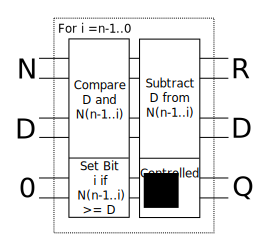
\includegraphics[width=0.9\textwidth]{images/division}
        \captionof{figure}{Binary Division Circuit.} \label{fig:div}
    \end{minipage}
    \medskip

    An interesting feature of this algorithm is that combined with an in-place
    adder\cite{CDKM:2004} it can easily be made partially in-place.  On
    \cref{line:intdiv:setToN} instead of allocating new space for $R(0)$ we can
    just use $N(i)$ as $R(0)$ since it will not be used again in the algorithm.
    In doing this we will overwrite the value of $N$ with $R$ as the algorithm
    is run.  The if statement on \cref{line:intdiv:compare} can be performed
    with a comparison circuit.  The result bit can be used to control the
    subtraction $R-D$.  The value of the result bit is the same as $Q(i)$ after
    the assignment on \cref{line:intdiv:setQ}, so $Q(i)$ can just be taken to
    be the result bit.  This avoids additional ancilla and the assignment to
    $Q(i)$.

    This divider uses a total of $n$ comparisons and subtractions of size $n$
    where $n$ is the bit width of the input. A comparison can be implemented by
    computing the highest order bit when the numbers are subtracted.

\section{Trigonometric functions with CORDIC}

    The CORDIC\cite{V:1959} algorithm was originally developed to calculate
    trigonometric functions on simple analog computers. Because of this the
    algorithms uses only simple operations such as bitshift, addition, and
    negation. Since these operations are simple to implement as reversible
    computations (and can in fact be done in-place) it is well suited for
    adaptation as a reversible algorithm. The basic idea of CORDIC is to apply
    repeated rotations which decrease in size with each iteration while using
    a comparator to choose the direction of each iteration such that they
    converge on the desired value (as shown in \cref{fig:cordic-rot}):

    \[ \theta = \alpha_0 + \alpha_1 + \dotsb + \alpha_{n-1} \]

    \begin{figure}
        \capstart
        \centering
        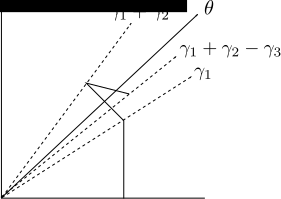
\includegraphics[width=.5\textwidth]{images/cordic-rot}
        \caption{Rotations are used to converge on $\theta$.}
        \label{fig:cordic-rot}
    \end{figure}

	The issue is that computing rotations is generally expensive; requiring
	multiplication and the evaluation of trig functions (the very thing we
	are using it to accomplish!). An important realization of the CORDIC
	method is that it is possible to choose rotation angles such that this
	problem is avoided.

        A rotation matrix is given by:
        \[
          R_i = \begin{bmatrix}
            \cos\gamma_i & -\sin\gamma_i \\
            \sin\gamma_i & \cos\gamma_i
          \end{bmatrix}
        \]
        Using trig identities we can simplify this to:
        \[
          R_i = K_i
                \begin{bmatrix}
                  1            & -\tan\gamma_i \\
                  \tan\gamma_i & 1
                \end{bmatrix}
        \]
        where $K_i = \frac{1}{\sqrt{1+\tan^2\gamma_i}}$.

        We can collect all the $K_i$ terms into a pre-computed scaling factor:
        \[ K(n) = \prod_{i=0}^{n-1}K_i \]
        This can be applied with a single multiplication after the computation is complete.

        We can select $\gamma_i = \tan^{-1}2^{-i}$ as our set of angles so that all multiplications can be done simply as bit shifts.
        These angles will be pre-computed
        All that is left to do is find the directions of rotation.
        We can approximate some angle $\theta$ with the iterative process: $\theta_{i+1} = \theta_i + \sigma_i\gamma_i$.
        We choose the rotation direction $\sigma$ by comparing $\theta_i$ with $\theta$.
        If $\theta_i$ is greater then $\theta$ we rotate in the negative direction.
        If $\theta_i$ is less then then $\theta$ we rotate in the positive direction.

        This iterative process can be stated as:
        \begin{equation}\label{eq:cordIter}
            \begin{aligned}
                x_{i+1}      &= x_i - \sigma_iy_i2^{-i}\\
                y_{i+1}      &= y_i + \sigma_ix_i2^{-i}\\
                \theta_{i+1} &= \theta_i - \sigma_i\gamma_i
            \end{aligned}
        \end{equation}

    \subsubsection{Reversible Implementation}

    The CORDIC algorithm can be implemented reversibly.
    %\todo{What is a reversible CORDIC useful for?}

	We pre-compute all of our rotation angles
	($\gamma_0,\gamma_1,\dotsc,\gamma_{n-1}$) as well as the scaling factor
	$K(n)$. Our input is the angle $\theta$ and our output is ($x$,$y$)
	where $\tan\theta = y/x$.

	\paragraph{Finding the directions of rotation} The directions of
	rotation can be determined using the sign bit of $\theta$.  At each step we
	copy out the sign bit of $\theta$ then add the angle $\gamma_i$ if $\theta$ is
	negative or subtract if it is positive.  At the end the copied out set of bits
	$\sigma$ determine the directions of rotation.  $\theta$ will approach zero so
	the higher order bits could possibly be cleaned up at the end of the step.
	Figure \ref{fig:CORDICDirections} shows a circuit for calculating $\sigma$.

	\begin{figure} 
            \capstart 
            \centering
	    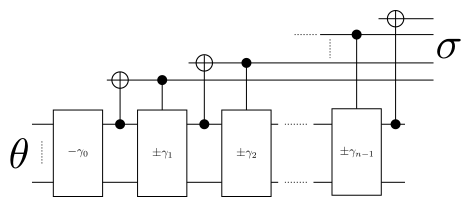
\includegraphics[width=\textwidth]{images/CORDICDirections} 

	    \caption{Circuit to determine directions of rotation.  The controls
            determine whether $\gamma$ is added or subtracted.}
            \label{fig:CORDICDirections} 

        \end{figure}

        \paragraph{Performing Rotations}

            The actual rotation section is done using the iterative process
            above (\cref{eq:cordIter}). This circuit is shown in
            \cref{fig:CORDICRotations}.

            \begin{figure}
                \capstart
                \centering
                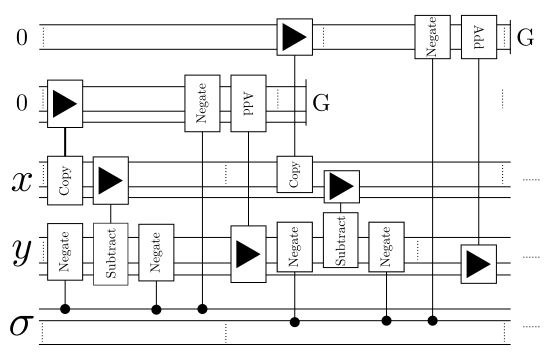
\includegraphics[width=\textwidth]{images/CORDICRotations}
                \caption{Circuit to perform rotations.
                         $x$ and $y$ are both initialized to $1/\sqrt{2}$.
                         Garbage is cleaned at the end by copying out the result and repeating the circuit.}
                \label{fig:CORDICRotations}
            \end{figure}
        \subsubsection{Analysis}
	\begin{figure}
                \capstart
                \centering
                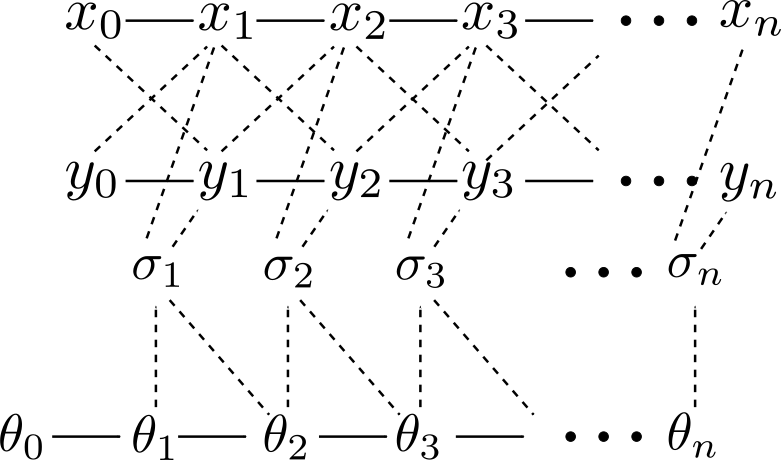
\includegraphics[width=0.9\textwidth]{images/CordicMDD}

                \caption{MDD for a reversible implementation of the CORDIC
                algorithm. Note that $x_0$ and $y_0$ are constants and
                $\theta_0$ is the input to the function.
                The $\sigma$ nodes are each one bit in size.}

                \label{fig:CordicMDD}
        \end{figure}

	Convergence of the CORDIC algorithm requires $O(n)$ rotations where $n$
	is the number of bits of precision required.  The cost of each rotation
	is also $O(n)$. This means the total cost of performing CORDIC is
	$O(n^2)$.

	If we were to allocate memory according to the naive method this would
	also mean a space used of $O(n^2)$ Instead an MDD pebble game is used
	to optimize this circuit.  The MDD for this implementation in shown in
	\cref{fig:CordicMDD}. On the top part of the diagram are modification
	chains for $x$ and $y$. The issue with these chains is that each new
	value is dependent on both of the previous values, i.e. $x_n+1$ depends
	on $x_n$ and $y_n$. This means that they cannot be both be advanced
	without leaving behind pebbles. We can choose to only leave pebbles
	behind on half the nodes, for example we can pebble $x_0,\dotsc,X_n$
	while advancing a single pebble along $y$. This however will only half
	the number of pebbles required.

	Assuming we pebble the $x$ chain and move the $y$ pebble forward as
	described above we can see the pebbles along the $x$ as a sort of 1D
	pebble game, we therefore can use the previously discussed strategies.
	With an incremental strategy we would only need to store
	$O(n^{\nicefrac{1}{2}})$ $x$ registers. This improves our overall space
	use to $O(n^{\nicefrac{3}{2}})$ while leaving our time complexity
	unchanged at $O(n^2)$.

	\Cref{fig:CORDICRotations} shows a possible generated circuit for the
	strategy where the $x$ chain is fully covered while the $y$ chain is
	advanced. As implied by the MDD this circuit can be partially
	parallelized with the circuit in \cref{fig:CORDICDirections}.

\section{Boolean Expressions}

AND operations can be reproduced using Toffoli gates onto ancilla:
\[
    \Qcircuit @C=1em @R=.7em {
        \lstick{a} & \ctrl{2}  & \rstick{a}\qw\\
        \lstick{b} & \ctrl{1}  & \rstick{b}\qw\\
        \lstick{0} & \targ     & \rstick{ab}\qw \\
    }
\]

XOR operations can be reproduced using two CNOT gates onto ancilla:
\[
    \Qcircuit @C=1em @R=.7em {
        \lstick{a} & \ctrl{2} & \qw      & \rstick{a}\qw\\
        \lstick{b} & \qw      & \ctrl{1} & \rstick{b}\qw\\
        \lstick{0} & \targ    & \targ    & \rstick{a \oplus b}\qw \\
    }
\]

Notice that AND operations are more costly both because they require a Toffoli gate rather then a CNOT gate,
and because they can only be applied through a XOR operation rather then directly.

One simple optimization is to notice that the Toffoli gate includes an XOR operation.
So we can calculate an expression such as $ab \oplus cd$ with:

\[
    \Qcircuit @C=1em @R=.7em {
        \lstick{a} & \ctrl{4} & \qw      & \rstick{a}\qw\\
        \lstick{b} & \ctrl{3} & \qw      & \rstick{b}\qw\\
        \lstick{c} & \qw      & \ctrl{2} & \rstick{c}\qw\\
        \lstick{d} & \qw      & \ctrl{1} & \rstick{d}\qw\\
        \lstick{0} & \targ    & \targ    & \rstick{ab \oplus cd}\qw \\
    }
\]

One method of generating quantum circuits from boolean expressions is to first transform them into circuits of NOT, XOR, and AND operations.
Given an expression with the recursive structure:

\begin{verbatim}
TERM = VAR
     | AND (TERM list)
     | XOR (TERM list)
     | NOT TERM
\end{verbatim}

An algorithm to produce a circuit for such an expression is given by:
%\todo{Boolean expression algorithm: Formally write this up}


\subsection{Converting OR to XOR}\cite{parent15}%\todo{Reference revs paper}
In the case of mutually exclusive statements XOR is equivalent to OR.
That is to say $a \lor b = a \oplus b$ if $a = 1 \implies b = 0$ and $b = 1 \implies a =0$.
For example $a\land b \lor \neg a \land c = a\land b \oplus \neg a \land c$.

This is very useful as it allows us to avoid the use of Toffoli gates and use less ancilla.
For example if we wished to compute $a \lor b \lor c$ we might use the circuit:

  \[
    \Qcircuit @C=1em @R=.7em {
        \lstick{a} & \ctrlo{3} & \qw      & \ctrlo{3} & \rstick{a}\qw\\
        \lstick{b} & \ctrlo{2} & \qw      & \ctrlo{2} & \rstick{b}\qw\\
        \lstick{c} & \qw       & \ctrlo{2}& \qw       & \rstick{c}\qw\\
        \lstick{0} & \targ     & \ctrl{1} & \targ     & \rstick{0}\qw \\
        \lstick{0} & \qw       & \targ    & \targ      & \rstick{a \lor b \lor c}\qw
    }
  \]

Where as $a \oplus b \oplus c$ can be computed as:

\[
    \Qcircuit @C=1em @R=.7em {
        \lstick{a} & \ctrl{3}  & \qw      & \qw      & \rstick{a}\qw\\
        \lstick{b} & \qw       & \ctrl{2} & \qw      & \rstick{b}\qw\\
        \lstick{c} & \qw       & \qw      & \ctrl{1} & \rstick{c}\qw\\
        \lstick{0} & \targ     & \targ    & \targ    & \rstick{a \oplus b \oplus c}\qw \\
    }
\]

Or if one of $a$, $b$, or $c$ are not needed in the later computation it can be done in-place as:

 \[
    \Qcircuit @C=1em @R=.7em {
        \lstick{a} & \ctrl{2}  & \qw      & \rstick{a}\qw\\
        \lstick{b} & \qw       & \ctrl{1} & \rstick{b}\qw\\
        \lstick{c} & \targ     & \targ    & \rstick{a \oplus b \oplus c}\qw \\
    }
\]

Given a set of AND expressions that are combined using OR we want to find sets of mutually exclusive statements that minimize the use of AND.
We consider each AND expression to be a vertex on a graph and add edges between vertices that are mutually exclusive.
Now we cover this graph using a minimum number of cliques.

After finding these cliques each set of mutually exclusive statements can be implemented by evaluating the AND statements and combining all of the values on a single ancilla using XOR for each clique.
These results can then be combined using OR statements (since OR is associative it does not matter how we group the statements).

%This algorithm has been implemented and tested on the BLIF benchmarks. 
%\todo{add reference and explain what BLIF is}
%The results are shown below:
%\todo{chart}

\section{Gray Code Controlled Counter\label{sec:findFirst}}
  Suppose you want to perform a set of functions which return some boolean value and you wish to know the first such function which returns $0$.
  For example if we have an $n$-bit number and we wish to find the position of the first $0$ value.

  In this case we want a controlled increment function that stop incrementing the first time the control is $0$.
  We therefore want to change the state of the counter by looking at just enough information to verify that all previous steps have been performed.
  To do this we must look at a subset whose value is unique to the previous step.
  Note some difficulty is introduced by the reversible nature of the circuit in that we cannot depend on parts of the state that we are updating.
  To do this we simply follow a binary counting method which flips one bit each step (Gray Code).
  Since only one bit is flipped per iteration the context of the unflipped bits is sufficient to verify the previous steps.
  An example of such a chain is shown below where the underlined portions of the state are the ones verified before the next step:
  \[
    000 \to 00\underline{1} \to 0\underline{1}1 \to 0\underline{10} \to \underline{1}10 \to
    \underline{1}1\underline{1} \to \underline{10}1 \to 100
  \]
  %A possible application of such a counter is in an input erasing multiplier.\todo{expand or remove}
